\documentclass{article}
\usepackage{amsfonts,amsmath,booktabs,adjustbox,float}
\usepackage{graphicx}
\graphicspath{.}
\title{Connect Four}
\author{Ahmed Ashraf}
\date{}
\begin{document}
\maketitle

\section{Herustic used}
 {
  \begin{equation*}
      V(cell,piece) = \begin{cases}
          100000  & \text{4 pieces of the same specified kind}              \\
          100     & \text{3 pieces of the specified kind and 1 empty tile}  \\
          1       & \text{2 pieces of the specified kind and 2 empty tiles} \\
          -80     & \text{3 pieces of the enemy piece and 1 empty tile}     \\
          -100000 & \text{4 piece of the enemy piece}
      \end{cases}
  \end{equation*}
 }

\subsection{Breakdown of the how the function will be used}
We will be itearting over the board, where each row,column, postively sloped diagonals, and negatively sloped diagonals are going to broken down into cells of length 4, and each cell will be evaluated individually. The Score returned from evaluated cells is going to be added to the global board Score.


\section{Data Structures used}
\begin{enumerate}
    \item \verb!ArrayList! to the store the valid location where the piece can be dropped
    \item \verb"TreeNode" A custom made data Structure that maintains a tree used for printing the MiniMax Tree.
    \item \verb"GameSettings" A data Structure from FXGL library that initialize the settings
    \item \verb"Input" used to get the input from the user e.g. the mouse position
    \item \verb"UserAction" defines the actions that can be made by the user.
    \item \verb"Color" controls the color of the piece in the GUI
    \item \verb"Entity" a FXGL data structure that is used to show Entities in the game GUI.
    \item \verb"EntityType" defines the type of the Entities that is going to be used in the game.
    \item \verb"Text" JavaFX data Structure that initialize a text that is going to displayed in the game UI.
    \item \verb"Map<String,Object> vars" initializes observalbe game variable.
    \item \verb"FXGLMenu" used to create a custom Main Menu.
    \item \verb"Rectangle" used to define the shape of the button in the main menu.
    \item \verb"Animation" used to build animation when the Rectangle is hovered over.
    \item \verb"Point2D" used to to track the mouse position.
\end{enumerate}
\subsection{Creating the Game GUI}
\begin{enumerate}
    \item \verb"createGUIBoard():void" creates the board in the game GUI.
    \item \verb"changeBallColor(Color color):void" Changes the ball color when the user has already played. It is redundent since there is no human second player.
\end{enumerate}
\subsection{Game Variables}
\begin{enumerate}
    \item {\small{\verb"PLAYER,AI,EMPTY"} }used to denote the piece in the terminal game board.
    \item {\small{\verb"TILE_SIZE"} }used to control the size of the Tile.
    \item {\small{\verb"SPEED"}} used to control the ball speed when the user uses the keyboard controls
    \item {\small{\verb"MAX_ROWS,MAX_COLS"}} controls the Rows and columns of the game board.
    \item {\small{\verb"MAX_WIDTH,MAX_HEIGHT"}} controls the size of window using the maximum rows and columns
    \item {\small{\verb"OFFSET"}} when creating the cells for evaluation there is an offset where if the iterator reaches the fiveth column it will case an out-of-bounds error.
    \item {\small{\verb"CELL_LENGTH"}} used to define the length of the cells. This variable was created to avoid Magic numbers
    \item {\small{\verb"terminalBoard:int[][]"}}\\ The main board which is going to updated througout the game runtime.
    \item {\small{\verb"boardTree"}} the tree that is going to be maintained throught the game runtime.
    \item {\small{\verb"playerScore,aiScore"}} Keeps track of the score of the game during its runtime.
\end{enumerate}
\subsection{Game functions}
\begin{enumerate}
    \item {\small\verb"createBoard():int[][]"}\\ creates an empty board.
    \item {\small\verb"dropPiece(int[][] board, int row, int col, int piece):void"} \\takes in the board,row,column, and the piece that is going to be drooped.
    \item {\small\verb"isValidLocation(int[][] board, int col):boolean"}\\takes in the board and the column and checks if the column has an empty space where the piece is going to be dropped.
    \item {\small\verb"getOpenRow(int[][] board, int col):int"} takes in the board and the column to get the next open row where the piece can be dropped.
    \item {\small\verb"printBoard(int[][] board):void"} prints the board in the terminal.
    \item {\small\verb"GameOver(int[][] board, int piece):boolean"} Classical check of the game. Checks if the and piece has a connect four
    \item {\small\verb"GameOver(int[][] board):boolean"} Custom check for the game where the game ends when there are no more valid locatoins
    \item {\small\verb"evaluateCell(int[] cell, int piece):int"} takes in the cell and the piece that is going to evaluated and returns the score.
    \item {\small\verb"connectFour(int[] cell, int piece):int"} takes in the cell and checks if there is a connect four
    \item {\small\verb"countPieces(int[] arr, int piece):int"} counts the pieces of the specified type in the cell.
    \item {\small\verb"scorePosition(int[][] board, int piece):int"} socres the game position for the game aiScore
    \item \verb"numberFours(int[][] board, int piece):int" counts the number of connect fours and updates the score of the game.
    \item {\small\verb"makeColArr(int[][] board, int c):int[]"} \\takes in the game board and the column and returns the column as an array
    \item {\small\verb"makeRowArr(int[][] board, int r):int[]"}\\ takes in the game board and the row and retusn the row as an array
    \item {\small\verb"isTerminalNode(int[][] terminalBoard):boolean"}\\classical check if the node is terminal
    \item {\small\verb"getValidLocations(int[][] board):ArrayList<Integer>"} takes in the board and returns the valid location where the piece can be dropped.
    \item {\footnotesize\verb"minimax(int[][] board, int depth, boolean maxPlayer, TreeNode node):int[]"}\\ implementes the minimax alogrithm and returns the column and score as an array where the column is index 0 and score is index 1. It takes as well the tree that is going to maintained throughout its run.
    \item {\small\texttt{minimax(int[][] board, int depth, int alpha,\\ int beta, boolean maxPlayer, TreeNode node):int[]}}\\implementes the minimax alogrithm with pruning.
    \item \verb"createGUIBoard():void" creats the gui board where the \verb"terminalBoard" is going to be used
\end{enumerate}
\subsection{Entity Factory}
The entity factory data structure is used to create the spawns or Entities at the correct loctaion during the game runtime
A tree data Structure was used to print the MiniMax Tree during its run. But the alogrithm can be implemented without a tree as it implementes depth-first search, where there is no need for tree to decrease memory usage.
\section{Libraries used}
\begin{enumerate}
    \item FXGL: Game engine library built upon JavaFX
    \item JavaFX
\end{enumerate}
\section{Sample runs}

\subsection{GUI}
\subsubsection{Main Menu}
\resizebox*{0.8\textwidth}{!}{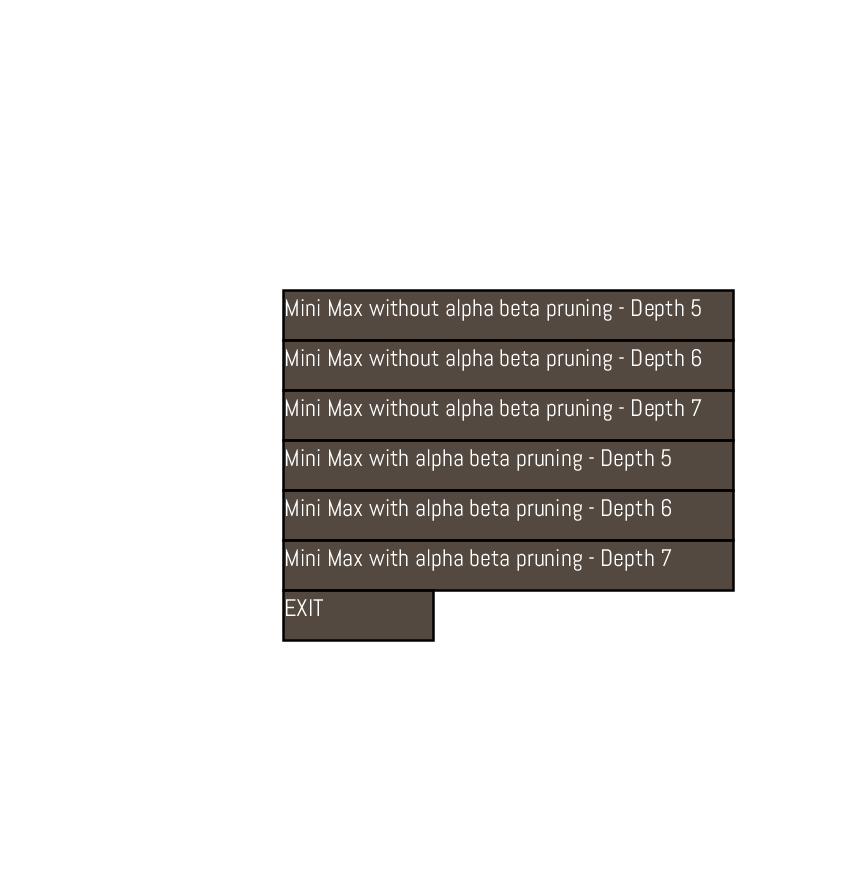
\includegraphics{MainMenuV2.png}}
\subsubsection{Game}
\resizebox*{0.45\textwidth}{!}{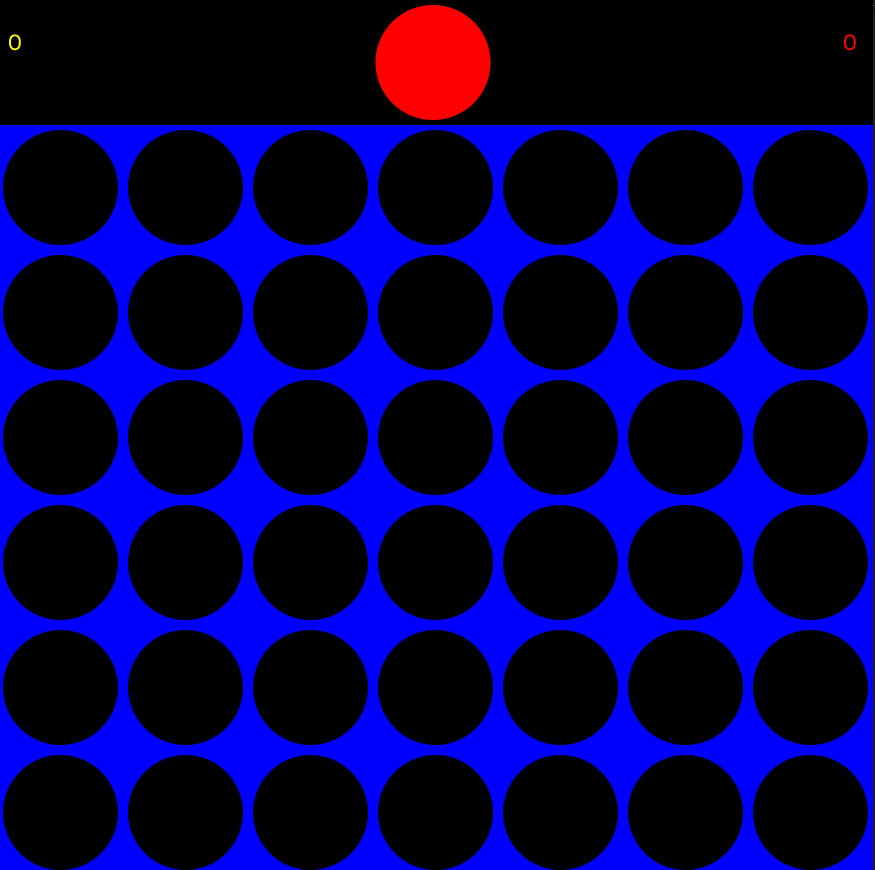
\includegraphics{Game1}}
\resizebox*{0.45\textwidth}{!}{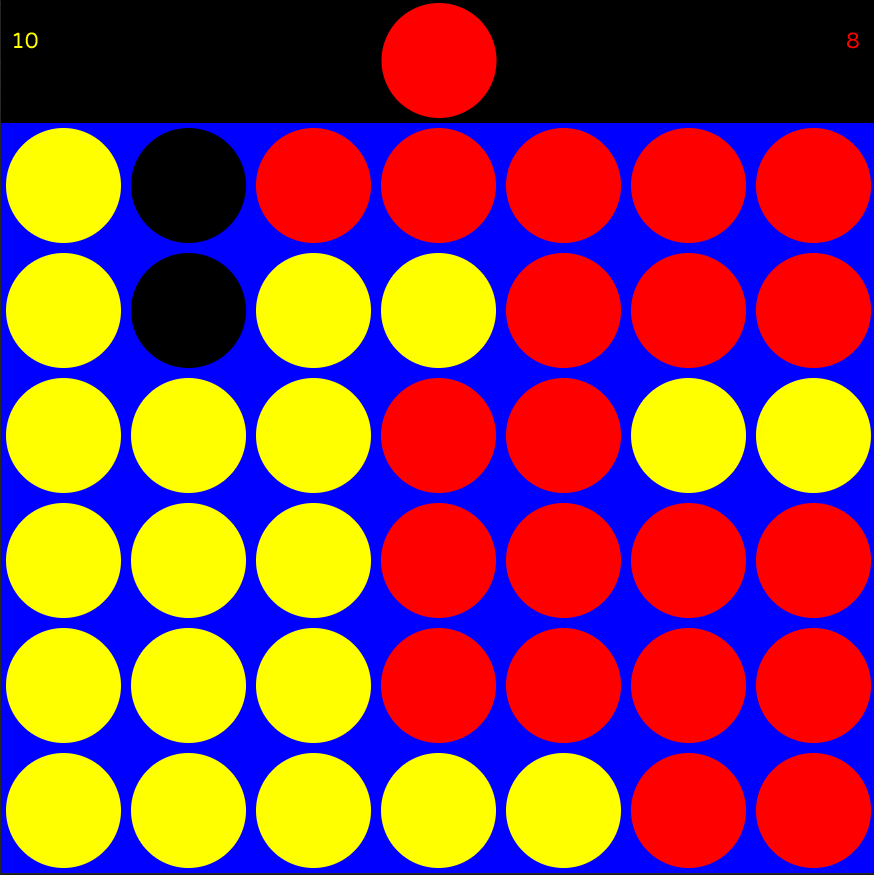
\includegraphics{Game2V2.png}}


\subsection{Mini Max Without \(\alpha-\beta\) pruning Depth 5}
We won't be able to show the whole tree since the tree is huge, so, we are showing parts of it not all of it.
We also will be showing only two turns.

The first turn.
\begin{verbatim}
The new Board after the player played : 
0	0	0	0	0	0	0	
0	0	0	0	0	0	0	
0	0	0	0	0	0	0	
0	0	0	0	0	0	0	
0	0	0	0	0	0	0	
0	0	0	0	0	0	1
2
|---  1
|  |---  2
|  |  |---  1
|  |  |  |---  1
|  |  |  |  |---  0
|  |  |  |  |---  1
|  |  |  |  |---  1
|  |  |  |  |---  1
|  |  |  |  |---  0
|  |  |  |  |---  0
|  |  |  |  |---  0
|  |  |  |---  1
.
.
.
Time Taken : 267.0 Millie Seconds
Nodes Expanded : 19607
Depth : 5
alpha beta : false
The new Board after AI Played : 
0	0	0	0	0	0	0	
0	0	0	0	0	0	0	
0	0	0	0	0	0	0	
0	0	0	0	0	0	0	
0	0	0	0	0	0	0	
0	2	0	0	0	0	1	
\end{verbatim}
The second turn.
\begin{verbatim}
The new Board after the player played : 
0	0	0	0	0	0	0	
0	0	0	0	0	0	0	
0	0	0	0	0	0	0	
0	0	0	0	0	0	0	
0	0	0	0	0	0	1	
0	2	0	0	0	0	1	
--------------------
5
|---  2
|  |---  23
|  |  |---  2
|  |  |  |---  101
|  |  |  |  |---  1
|  |  |  |  |---  3
|  |  |  |  |---  101
|  |  |  |  |---  101
|  |  |  |  |---  2
|  |  |  |  |---  1
|  |  |  |  |---  1
|  |  |  |---  101
.
.
.
Time Taken : 266.0 Millie Seconds
Nodes Expanded : 19606
Depth : 5
alpha beta : false
The new Board after AI Played : 
0	0	0	0	0	0	0	
0	0	0	0	0	0	0	
0	0	0	0	0	0	0	
0	0	0	0	0	0	0	
0	0	0	0	0	0	1	
0	2	2	0	0	0	1	
--------------------
\end{verbatim}
The final turn
\begin{verbatim}
2147483647
|---  2147483647

Time Taken : 0.0 Millie Seconds
Nodes Expanded : 1
Depth : 5
alpha beta : false
The new Board after AI Played : 
2	1	1	1	1	1	1	
2	1	1	1	2	1	2	
2	2	1	2	1	2	1	
2	2	2	2	1	1	1	
2	2	2	2	1	1	1	
2	2	2	2	2	1	1	
--------------------
Player 2 Wins
Average time : 27.88095238095238
Average nodes expanded : 3357
\end{verbatim}

\subsection{Mini Max with \(\alpha-\beta\) pruning-Depth 5}
The first turn
\begin{verbatim}
    The new Board after the player played : 
0	0	0	0	0	0	0	
0	0	0	0	0	0	0	
0	0	0	0	0	0	0	
0	0	0	0	0	0	0	
0	0	0	0	0	0	0	
0	0	0	0	0	0	1	
--------------------
2
|---  1:1:2147483647
|  |---  2:-2147483648:2
|  |  |---  1:1:2147483647
|  |  |  |---  1:-2147483648:1
|  |  |  |  |---  0:0:2147483647
|  |  |  |  |---  1:1:2147483647
|  |  |  |  |---  1:1:2147483647
|  |  |  |  |---  1:1:2147483647
|  |  |  |  |---  1:1:2147483647
|  |  |  |  |---  1:1:2147483647
|  |  |  |  |---  1:1:2147483647
|  |  |  |---  1:-2147483648:1
|  |  |  |---  1:-2147483648:1
|  |  |  |---  1:-2147483648:1
|  |  |  |---  1:-2147483648:1
|  |  |  |---  1:-2147483648:1
|  |  |  |---  1:-2147483648:1
|  |  |---  2:2:2147483647
.
.
.
Time Taken : 49.0 Millie Seconds
Nodes Expanded : 1501
Depth : 5
alpha beta : true
The new Board after AI Played : 
0	0	0	0	0	0	0	
0	0	0	0	0	0	0	
0	0	0	0	0	0	0	
0	0	0	0	0	0	0	
0	0	0	0	0	0	0	
0	2	0	0	0	0	1	
--------------------
\end{verbatim}
The second turn
\begin{verbatim}
    The new Board after the player played : 
0	0	0	0	0	0	0	
0	0	0	0	0	0	0	
0	0	0	0	0	0	0	
0	0	0	0	0	0	0	
0	0	0	0	0	0	1	
0	2	0	0	0	0	1	
--------------------
5
|---  2:2:2147483647
|  |---  23:-2147483648:23
|  |  |---  2:2:2147483647
|  |  |  |---  101:-2147483648:101
|  |  |  |  |---  1:1:2147483647
|  |  |  |  |---  3:3:2147483647
|  |  |  |  |---  101:101:2147483647
|  |  |  |  |---  101:101:2147483647
|  |  |  |  |---  101:101:2147483647
|  |  |  |  |---  101:101:2147483647
|  |  |  |  |---  101:101:2147483647
|  |  |  |---  101:-2147483648:101
|  |  |  |  |---  2:2:101
|  |  |  |  |---  2:2:101
|  |  |  |---  2:-2147483648:2
.
.
.
Time Taken : 74.0 Millie Seconds
Nodes Expanded : 2359
Depth : 5
alpha beta : true
The new Board after AI Played : 
0	0	0	0	0	0	0	
0	0	0	0	0	0	0	
0	0	0	0	0	0	0	
0	0	0	0	0	0	0	
0	0	0	0	0	0	1	
0	2	2	0	0	0	1	
--------------------
\end{verbatim}
The final turn
\begin{verbatim}
Time Taken : 0.0 Millie Seconds
Nodes Expanded : 0
Depth : 5
alpha beta : true
The new Board after AI Played : 
2	1	1	1	1	1	1	
2	1	1	1	2	1	2	
2	2	1	2	1	2	1	
2	2	2	2	1	1	1	
2	2	2	2	1	1	1	
2	2	2	2	2	1	1	
--------------------
Player 2 Wins
Average time : 10.261904761904763
Average nodes expanded : 787
\end{verbatim}

\section{Comparsion between MiniMax with pruning and Without pruning}
\subsection{At depth 5}

\begin{table}[H]
    \caption{Depth 5}
    \centering
    \begin{tabular}{c c c c c}
        \toprule
                & \multicolumn{2}{c}{With Pruning} & \multicolumn{2}{c}{Without Pruning}                  \\
        \cmidrule{2-3}
        \cmidrule{4-5}
        Turn    & Time                             & Nodes                               & Time  & nodes  \\
        \midrule
        1       & 47.0                             & 1501                                & 363.0 & 19607  \\
        2       & 79.0                             & 2359                                & 209.0 & 19606  \\
        3       & 31.0                             & 4028                                & 97.0  & 19575  \\
        4       & 25.0                             & 3390                                & 85.0  & 19190  \\
        5       & 18.0                             & 2244                                & 42.0  & 9330   \\
        6       & 10.0                             & 620                                 & 45.0  & 9330   \\
        7       & 33.0                             & 2726                                & 47.0  & 9329   \\
        8       & 31.0                             & 4746                                & 64.0  & 9302   \\
        9       & 11.0                             & 2202                                & 41.0  & 7615   \\
        10      & 9.0                              & 1625                                & 15.0  & 3903   \\
        11      & 27.0                             & 2494                                & 14.0  & 3901   \\
        12      & 9.0                              & 1876                                & 27.0  & 3859   \\
        13      & 13.0                             & 1716                                & 12.0  & 3505   \\
        14      & 15.0                             & 753                                 & 5.0   & 1242   \\
        15      & 1.0                              & 410                                 & 24.0  & 892    \\
        16      & 1.0                              & 167                                 & 1.0   & 349    \\
        17      & 1.0                              & 103                                 & 1.0   & 289    \\
        18      & 1.0                              & 105                                 & 1.0   & 167    \\
        19      & 0.0                              & 5                                   & 0.0   & 33     \\
        20      & 0.0                              & 2                                   & 0.0   & 8      \\
        21      & 0.0                              & 0                                   & 0.0   & 1      \\
        \midrule
        Average & 17.24                            & 1574.9                              & 51.5  & 6715.9 \\
        \bottomrule
    \end{tabular}
\end{table}

\begin{table}[H]
    \caption{At Depth 6}
    \centering
    \begin{tabular}{c c c c c}
        \toprule
                & \multicolumn{2}{c}{With Pruning} & \multicolumn{2}{c}{Without Pruning}                    \\
        \cmidrule{2-3}
        \cmidrule{4-5}
        Turn    & Time                             & Nodes                               & Time  & nodes    \\
        \midrule
        1       & 120.0                            & 4643                                & 861.0 & 137255   \\
        2       & 110.0                            & 8395                                & 580.0 & 137217   \\
        3       & 273.0                            & 53938                               & 603.0 & 136609   \\
        4       & 27.0                             & 3907                                & 624.0 & 110069   \\
        5       & 19.0                             & 4265                                & 181.0 & 55953    \\
        6       & 28.0                             & 5476                                & 189.0 & 55951    \\
        7       & 18.0                             & 2004                                & 371.0 & 55519    \\
        8       & 89.0                             & 5272                                & 389.0 & 52347    \\
        9       & 8.0                              & 1586                                & 137.0 & 39070    \\
        10      & 5.0                              & 1026                                & 45.0  & 13195    \\
        11      & 16.0                             & 1620                                & 21.0  & 5439     \\
        12      & 32.0                             & 1561                                & 72.0  & 5287     \\
        13      & 16.0                             & 1681                                & 55.0  & 4643     \\
        14      & 6.0                              & 1187                                & 13.0  & 3075     \\
        15      & 6.0                              & 596                                 & 4.0   & 1005     \\
        16      & 2.0                              & 396                                 & 6.0   & 783      \\
        17      & 2.0                              & 258                                 & 3.0   & 376      \\
        18      & 2.0                              & 214                                 & 1.0   & 244      \\
        19      & 0.0                              & 5                                   & 1.0   & 19       \\
        20      & 0.0                              & 1                                   & 0.0   & 3        \\
        21      & 0.0                              & 0                                   & 0.0   & 1        \\
        \midrule
        Average & 37.1                             & 4668.14                             & 197.9 & 38764.76 \\
        \bottomrule
    \end{tabular}
\end{table}
\end{document}